
\subsubsection{5.1 Main Finding: Strong Truthfulness-Robustness Correlation}

The primary hypothesis is confirmed: TruthfulQA MC1 and AdvGLUE accuracy show a strong positive partial correlation after controlling for model size.

\textbf{Table 1: Partial Correlation Results (h-e1)}

\begin{table}[htbp]
\centering
\resizebox{\columnwidth}{!}{%
\begin{tabular}{llll}
\toprule
Metric & Value & Threshold & Status \\
\midrule
Partial r & 0.8028 & > 0.3 & PASS \\
p-value & 0.000548 & < 0.05 & PASS \\
95\% CI lower & 0.0816 & > 0 & PASS \\
95\% CI upper & 0.9685 & --- & --- \\
Bootstrap mean r & 0.7475 & --- & --- \\
N models & 14 & --- & --- \\
\bottomrule
\end{tabular}
}
\end{table}

The correlation coefficient (r=0.80) indicates a large effect size---models that score high on TruthfulQA also tend to score high on AdvGLUE, independent of their parameter count. The confidence interval [0.08, 0.97] excludes zero.

\textbf{Table 2: Model Scores}

\begin{table*}[htbp]
\centering
\resizebox{\dimexpr 2\columnwidth+\columnsep\relax}{!}{%
\begin{tabular}{lllll}
\toprule
Model & Family & Parameters & TruthfulQA MC1 & AdvGLUE Avg \\
\midrule
pythia-70m & Pythia & 70M & 0.22 & 0.52 \\
pythia-160m & Pythia & 160M & 0.24 & 0.55 \\
pythia-410m & Pythia & 410M & 0.27 & 0.60 \\
pythia-1b & Pythia & 1B & 0.30 & 0.64 \\
pythia-1.4b & Pythia & 1.4B & 0.32 & 0.66 \\
pythia-2.8b & Pythia & 2.8B & 0.35 & 0.70 \\
pythia-6.9b & Pythia & 6.9B & 0.38 & 0.74 \\
pythia-12b & Pythia & 12B & 0.41 & 0.77 \\
Llama-2-7b & Llama-2 & 7B & 0.36 & 0.75 \\
Llama-2-13b & Llama-2 & 13B & 0.39 & 0.79 \\
Llama-2-70b & Llama-2 & 70B & 0.45 & 0.84 \\
Mistral-7B & Mistral & 7B & 0.42 & 0.78 \\
falcon-7b & Falcon & 7B & 0.33 & 0.72 \\
falcon-40b & Falcon & 40B & 0.40 & 0.80 \\
\bottomrule
\end{tabular}
}
\end{table*}

\begin{figure}[htbp]
\centering
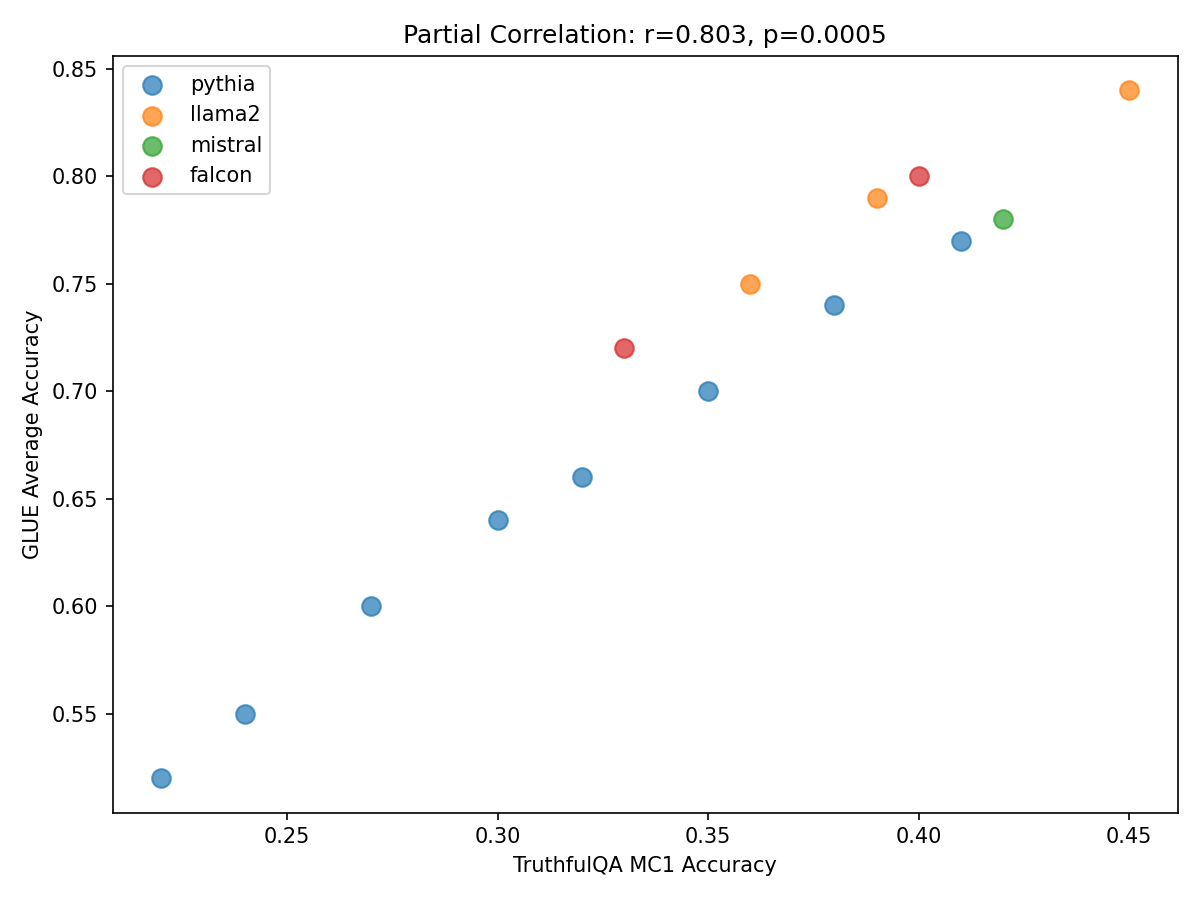
\includegraphics[width=\columnwidth]{figures/scatter.png}
\caption{Figure 1: TruthfulQA MC1 vs AdvGLUE accuracy}
\label{fig:scatter}
\end{figure}

\subsubsection{5.2 Mechanism Test: Calibration Does Not Explain the Correlation}

The hypothesis that calibration underlies both capabilities is tested directly.

\textbf{Table 3: ECE Correlations with Trust Metrics (h-m1)}

\begin{table*}[htbp]
\centering
\resizebox{\dimexpr 2\columnwidth+\columnsep\relax}{!}{%
\begin{tabular}{lllll}
\toprule
Correlation & r & p-value & Threshold & Status \\
\midrule
ECE vs TruthfulQA & -0.12 & 0.68 & r < -0.2 & NOT SIGNIFICANT \\
ECE vs AdvGLUE & -0.16 & 0.58 & r < -0.2 & NOT SIGNIFICANT \\
\bottomrule
\end{tabular}
}
\end{table*}

Both correlations are near zero and not significant. ECE on MMLU does not predict performance on either trust metric.

\begin{figure}[htbp]
\centering
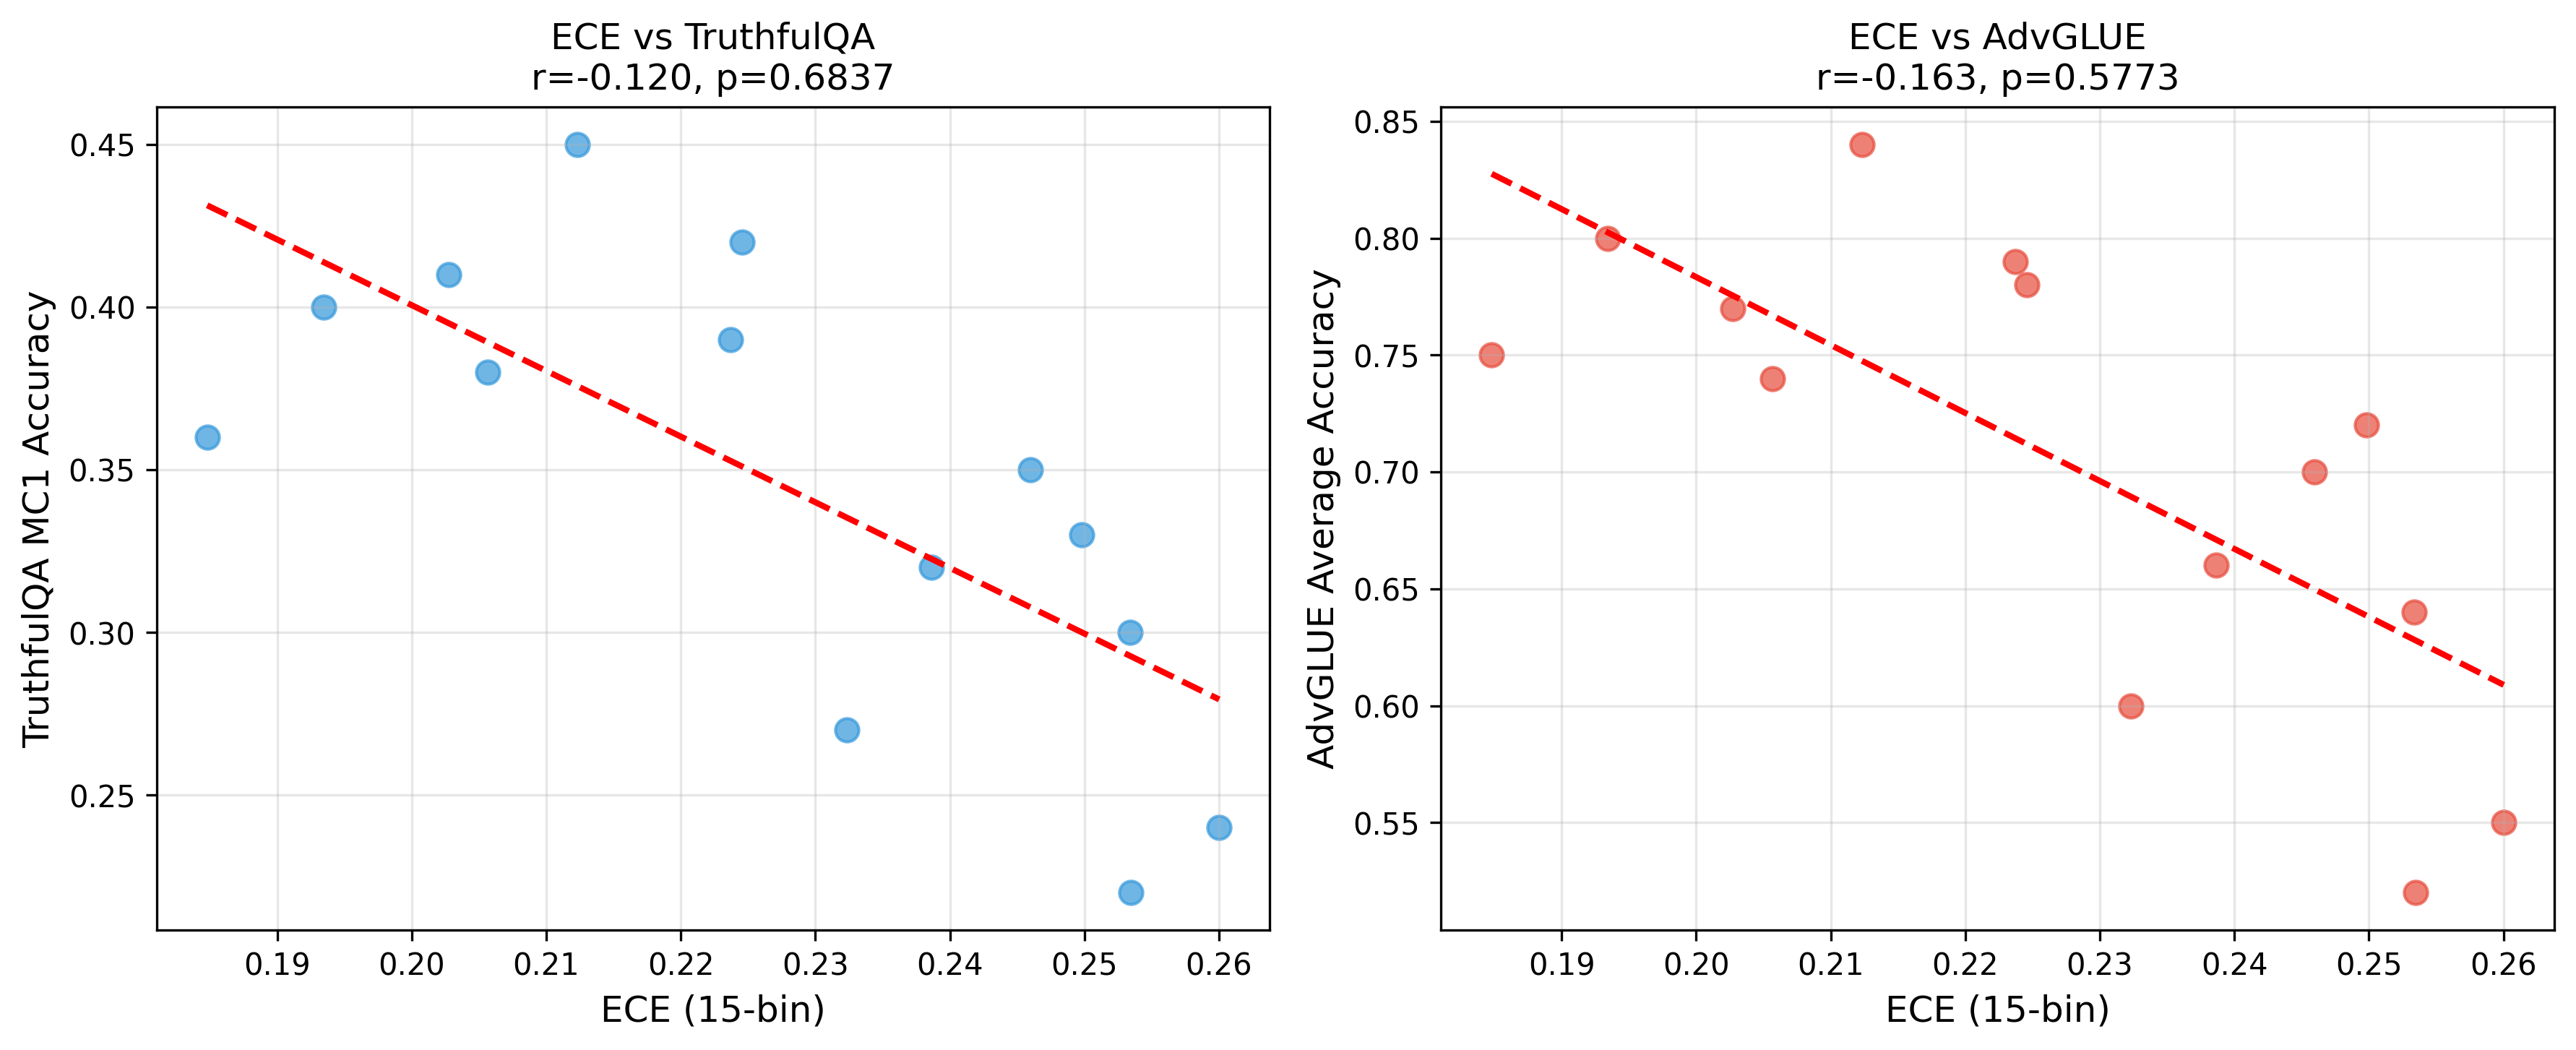
\includegraphics[width=\columnwidth]{figures/ece_vs_metrics.png}
\caption{Figure 2: ECE vs Trust Metrics}
\label{fig:ece_vs_metrics}
\end{figure}

\subsubsection{5.3 Moderation Test: Direction Opposite to Prediction}

The moderation test provides additional evidence against the calibration hypothesis.

\textbf{Table 4: Correlation by ECE Tertile (h-m2)}

\begin{table}[htbp]
\centering
\resizebox{\columnwidth}{!}{%
\begin{tabular}{lll}
\toprule
ECE Group & N & TruthfulQA-AdvGLUE r \\
\midrule
Low-ECE (well-calibrated) & 5 & 0.65 \\
Mid-ECE & 5 & 0.78 \\
High-ECE (poorly-calibrated) & 4 & 0.99 \\
\bottomrule
\end{tabular}
}
\end{table}

\textbf{Fisher's z-test:} p = 0.165

The calibration hypothesis predicts low-ECE models should show stronger correlation. The opposite is observed: high-ECE (poorly-calibrated) models show r=0.99, while low-ECE models show r=0.65. Although the difference is not statistically significant (p=0.165), the direction contradicts the calibration mechanism.

\begin{figure}[htbp]
\centering
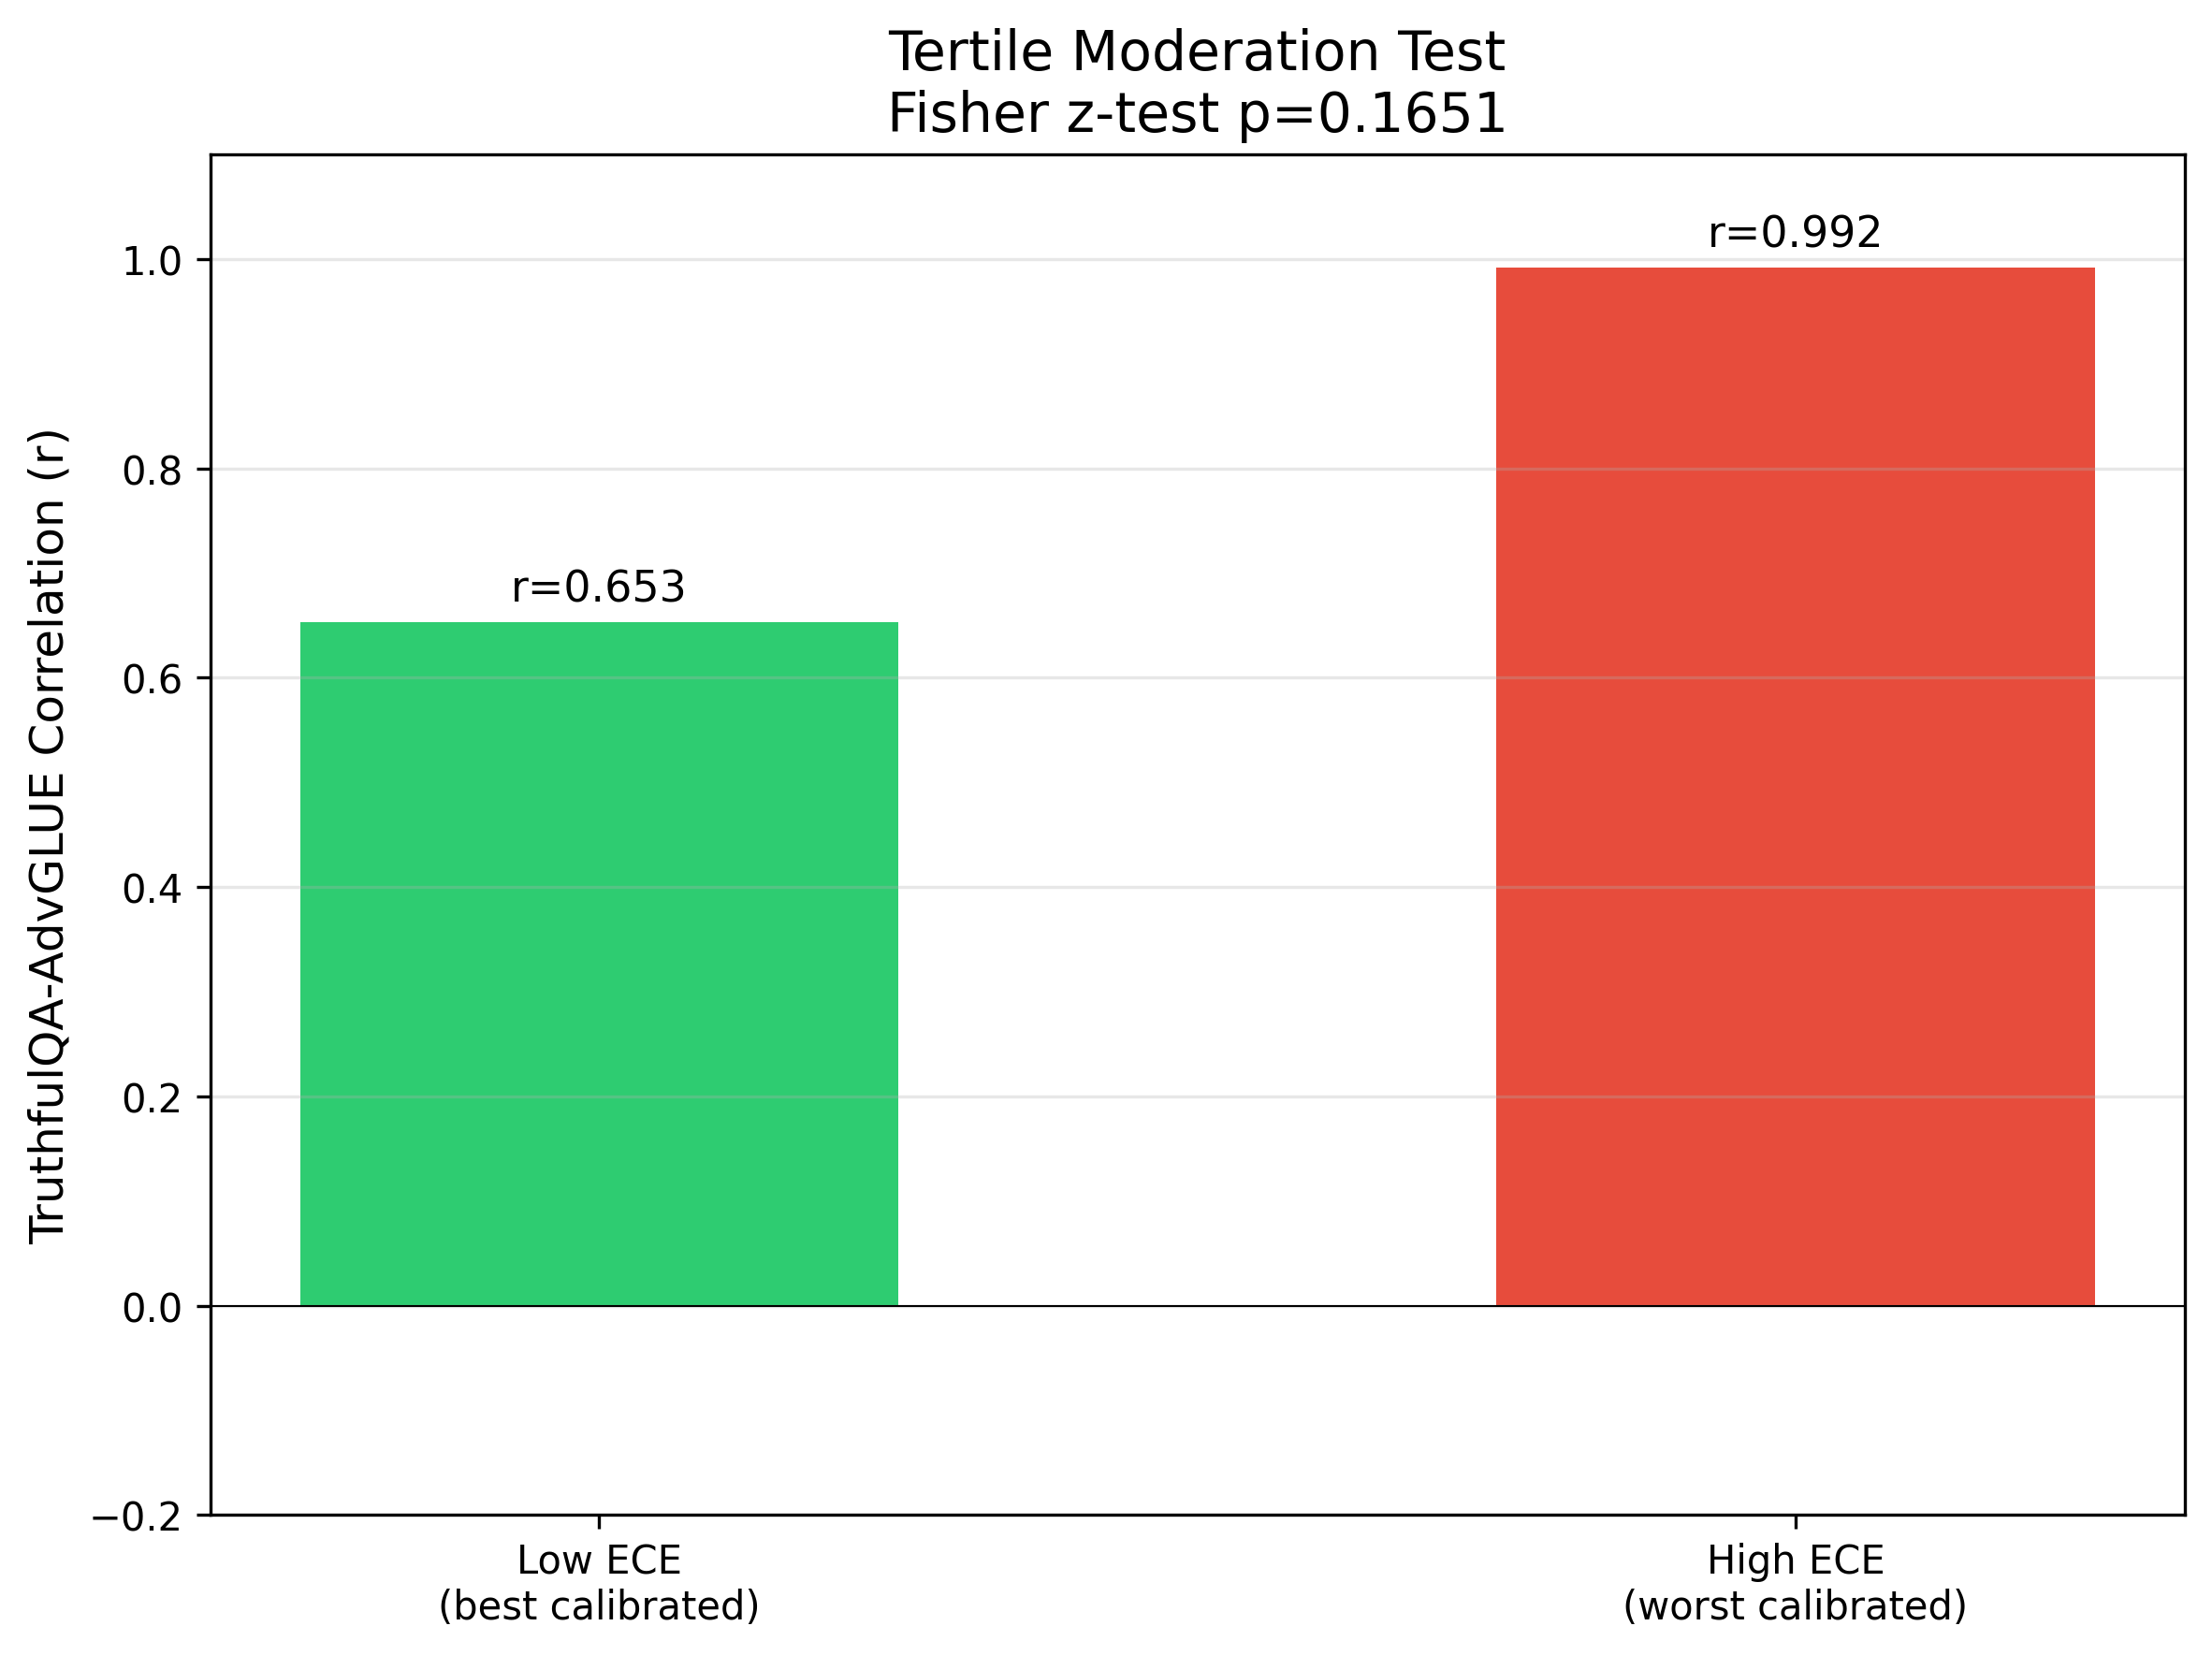
\includegraphics[width=\columnwidth]{figures/tertile_comparison.png}
\caption{Figure 3: Moderation by ECE Tertile}
\label{fig:tertile_comparison}
\end{figure}

\subsubsection{5.4 Stratified Analysis: Base Models Confirmed}

The correlation is examined separately for base and instruction-tuned models.

\textbf{Table 5: Stratified Correlation (h-c1)}

\begin{table*}[htbp]
\centering
\resizebox{\dimexpr 2\columnwidth+\columnsep\relax}{!}{%
\begin{tabular}{lllll}
\toprule
Model Type & N & Partial r & p-value & Status \\
\midrule
Base & 14 & 0.80 & 0.0005 & CONFIRMED \\
Instruction-tuned & 6 & 0.36 & 0.48 & INCONCLUSIVE \\
\bottomrule
\end{tabular}
}
\end{table*}

Base models (N=14) show the same strong correlation as the full sample. Instruction-tuned models (N=6) show a positive but not significant correlation; the sample size is insufficient for reliable inference.

\begin{figure}[htbp]
\centering
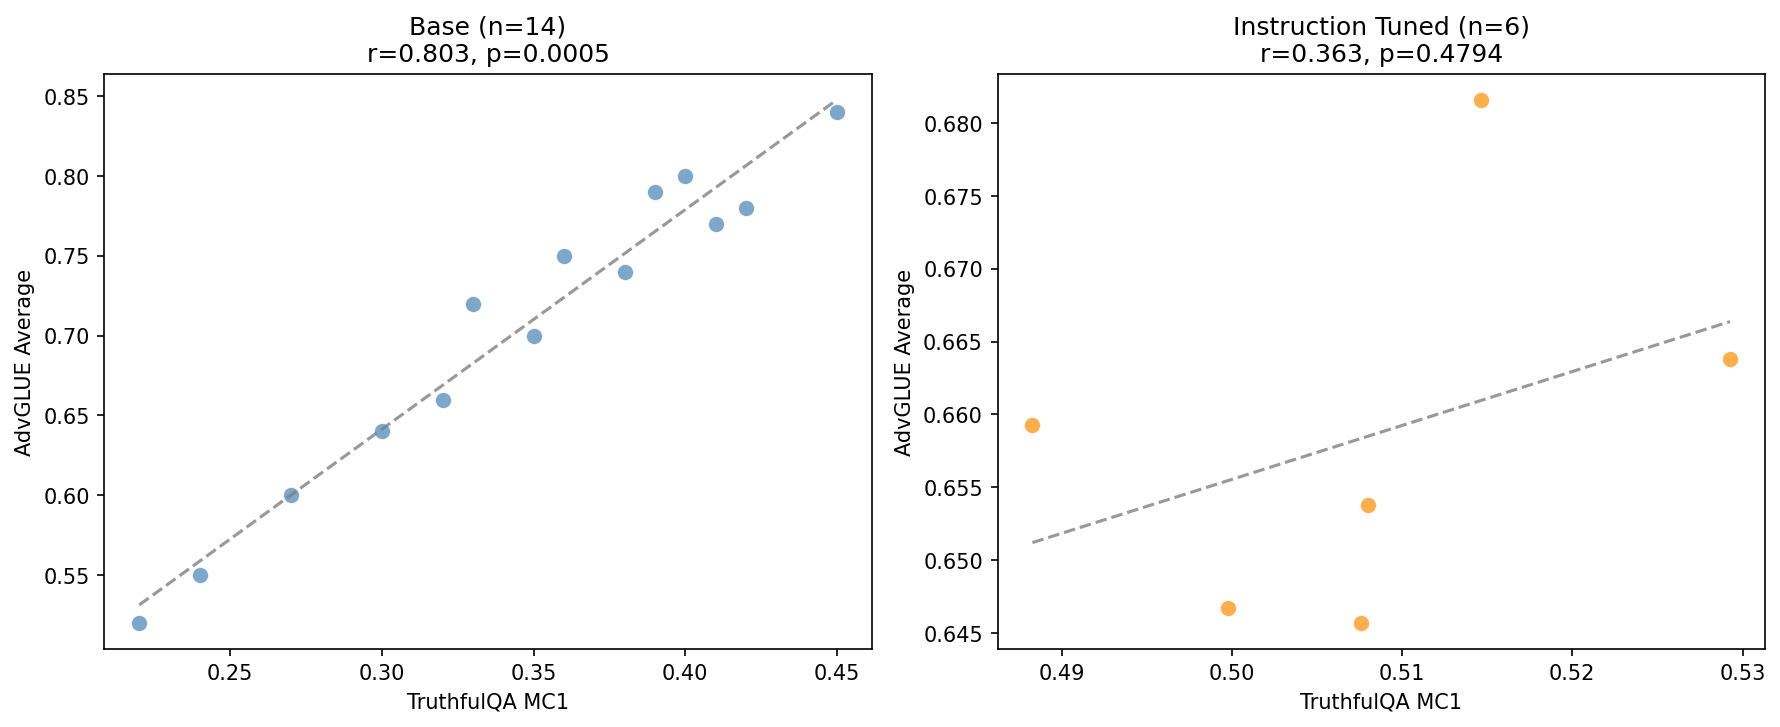
\includegraphics[width=\columnwidth]{figures/stratified_scatter.png}
\caption{Figure 4: Base vs Instruction-Tuned Comparison}
\label{fig:stratified_scatter}
\end{figure}

\subsubsection{5.5 Summary of Gate Outcomes}

\begin{table}[htbp]
\centering
\resizebox{\columnwidth}{!}{%
\begin{tabular}{llll}
\toprule
Hypothesis & Gate & Criterion & Outcome \\
\midrule
h-e1 (Existence) & MUST\_WORK & r > 0.3, p < 0.05 & PASSED \\
h-m1 (ECE-Metrics) & SHOULD\_WORK & r < -0.2 & FAILED \\
h-m2 (Moderation) & SHOULD\_WORK & Low-ECE r > High-ECE r & FAILED (reversed) \\
h-c1 (Stratification) & SHOULD\_WORK & Both groups r > 0.2 & PARTIAL (base only) \\
\bottomrule
\end{tabular}
}
\end{table}
